\chapter{Solução Proposta}
\label{cap:solucao}


Neste capítulo, nós apresentamos a arquitetura e aspectos de implementação do \choreos \ee (EE).   
Incluímos na descrição os pontos de extensão do arcabouço, e destacamos
como as decisões arquiteturais e de implementação auxiliam o implantador
a superar os desafios presentes na implantação de coreografia de grande escala.

Para a implementação do arcabouço Enactment Engine contribuíram Daniel Cuckier, Carlos Eduardo do Santos, Felipe Pontes, Alfonso Diaz, Nelson Lago, Paulo Moura, Thiago Furtado e demais colegas dos projetos Baile e CHOReOS. O \ee é software livre 
sob a Licença Pública da Mozilla 2\footnote{\url{http://www.mozilla.org/MPL/2.0/}} 
e está disponível em \url{http://ccsl.ime.usp.br/enactmentengine}. 

Alguns aspectos aqui discutidos serão o tratados em alto nível,
priorizando o que é importante para o entendimento das contribuições
acadêmicas deste trabalho.
Detalhes de mais baixo nível sobre nosso middleware, principalmente do ponto de vista do
usuário, podem ser encontrados no \userguide.

Conforme já anunciado no Capítulo~\ref{cap:implantacao},
lembramos que para as descrições que se seguem utilizaremos
termos técnicos como definidos no DEPL~\cite{DEPL2006}.

\section{Arquitetura}

A arquitetura do \ee é exibida na Figura~\ref{fig:arquitetura}.

\begin{figure}[ht]
\centering
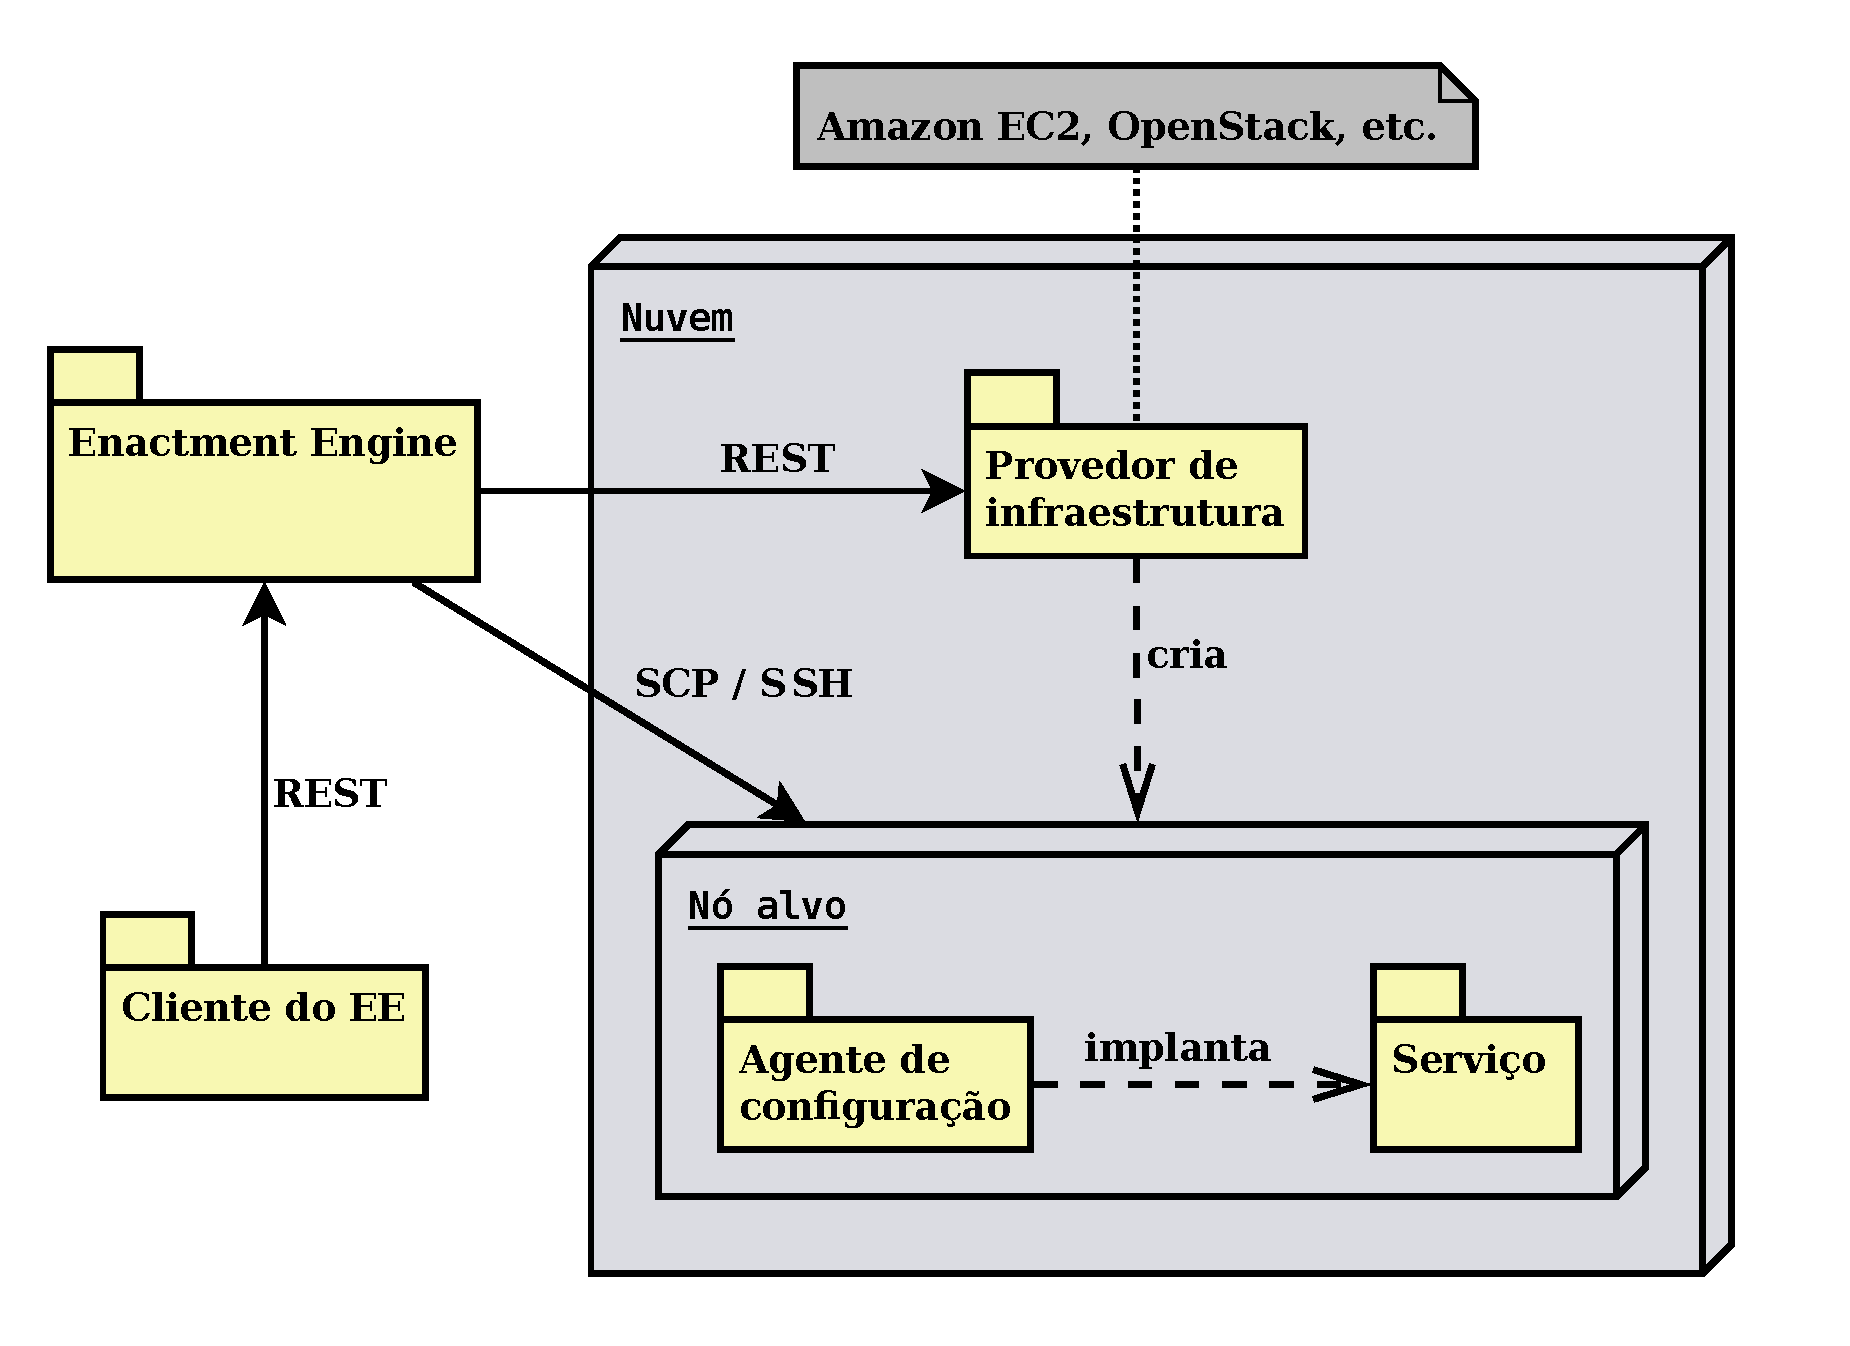
\includegraphics[width=0.7\linewidth]{arquitetura.pdf}
\caption{Arquitetura do \choreos \ee.}
\label{fig:arquitetura}
\end{figure}

\begin{itemize}

\item O \emph{Cloud Gateway} é um serviço de terceiros capaz de criar e destruir máquinas virtuais 
(também chamadas de \emph{nós}), normalmente em um ambiente de computação em nuvem. 
Atualmente o \ee suporta o Amazon EC2 e o OpenStack.

\item O \emph{agente de configuração} é executado nos nós alvos
e dispara os scripts que implementam as fases de preparação
e inicialização da implantação dos serviços.
O \ee utiliza o Chef Solo\footnote{\url{http://docs.opscode.com/chef_solo.html}}
como seu agente de configuração.

\item O \emph{cliente do \ee} é um programa ou script desenvolvido
pelo implantador, onde a especificação da coreografia é definida.
Esse script deve enviar a especificação da coreografia para o \ee
através das operações REST fornecidas pelo \ee.
Uma opção para implementar essas chamadas é utilizar
a biblioteca Java por nós fornecidas, que abstrai os detalhes
das chamadas REST.

\item O \emph{\ee} implanta os serviços da coreografia
com base na especificação enviada pelo cliente.
O processo implementado pelo \ee para efetuar a implementação
é descrito na Figura~\ref{fig:processo}, e explicado logo em seguida. 
\todo{explicar q é um serviço, mas q deve ser instalado}

\end{itemize} 

A Figura~\ref{fig:processo} exibe o processo de implantação de composições
de serviços implementado pelo \ee:

\begin{figure}[ht]
\centering
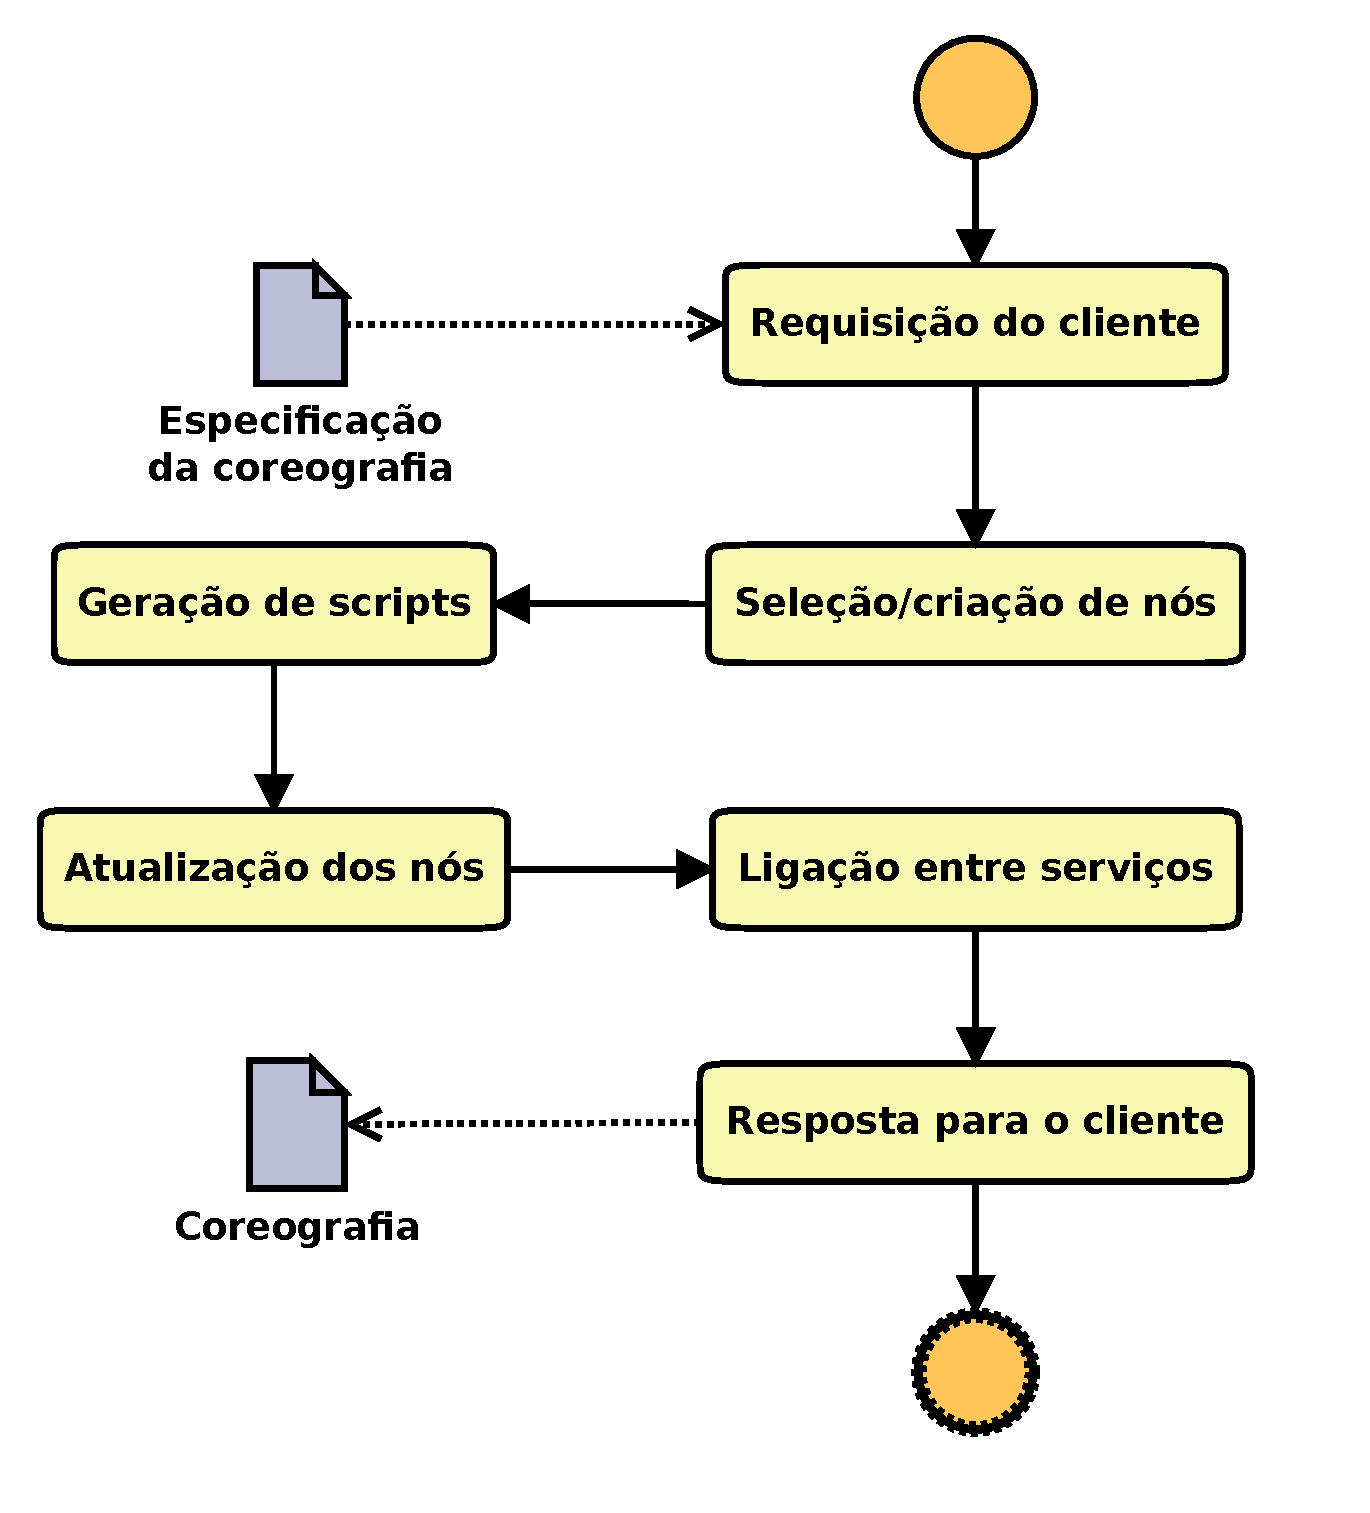
\includegraphics[width=0.5\textwidth]{processo.pdf}
\caption{Processo de implantação implementado pelo \ee.}
\label{fig:processo}
\end{figure}

\begin{enumerate}

\item \emph{Requisição do cliente:} o EE recebe a especificação da coreografia a ser implantada.
O formato dessa especificação é descrito na Seção~\ref{sec:spec}.

\item \emph{Seleção/criação de nós}: para cada serviço especificado, o EE seleciona um ou mais nós 
onde o serviço será implantado (um serviço pode ter várias réplicas implantadas). 
Se preciso, o EE requisitará ao Cloud Gateway a criação de novos nós.
Esse processo de seleção/criação de nós pode levar em conta os requisitos não-funcionais
dos serviços a serem implantados.
A política de seleção de nós é extensível, sendo definida pela organização
gerenciadora da instância do EE em execução. Algumas políticas já fornecidas são
``sempre cria um novo nó'' e ``cria novos nós até um certo limite, depois faz rodízio entre eles''.
Mais informações sobre a extensibilidade da política de seleção
são fornecidas na Seção~\ref{sec:extensao}.

\item \emph{Geração de scripts}: para cada serviço da coreografia, o EE gera dinamicamente os scripts de configuração do ambiente e inicialização do serviço. 
O EE configura então o agente de configuração do nó alvo para aquele serviço 
para que o script seja executado.

\item \emph{Atualização dos nós}: para cada nó alvo que receberá serviços da coreografia,
o EE dispara a execução do agente de configuração, de forma que o serviço é efeticamente
implantado e inicializado no nó.

\item \emph{Ligação entre serviços}: após os serviços terem sido iniciados, 
para cada relação de dependência na coreografia (ex: serviço \textsf{TravelAgency}
depende do serviço \textsf{Airline}), o EE fornece o endereço da dependência 
(ex: \url{http://airline.com/ws}) ao serviço dependente.
Mais informações sobre o processo de ligação são fornecidas na Seção~\ref{sec:ligacao}.
A implementação padrão para efetivar a ligação entre serviços, é a invocação de uma
operação SOAP, denominada \texttt{setInvocationAddress} no serviço dependente. 
Esse comportamento padrão pode ser modificado por extensão do EE,
conforme explicado adiante na Seção~\ref{sec:extensao}.

\item \emph{Resposta para o cliente}: o EE responde ao seu cliente,
fornecendo informações sobre em que nó cada serviço foi implantado,
e as URIs de acesso a cada serviço da coreografia.
O formato da resposta é descrito na Seção~\ref{sec:spec}.

\end{enumerate}

Há também alguns outros passos opcionais que não são aqui descrito por estarem fora
do escopo deste trabalho. Um exemplo é a implantação da infra-estrutura de monitoramento
dos nós alvos. O agente de monitoramento 
(Ganglia\footnote{\url{http://ganglia.sourceforge.net}})
é implantado nos nós alvos pelo EE e
coleta valores de uso de CPU, memória e disco dos nós.
\todo{para onde isso é enviado?}

\section{Especificação da coreografia}
\label{sec:spec}

\section{Ligação entre serviços}
\label{sec:ligacao}

Segundo Dearle~\cite{Dearle2007PastPresentFuture}, componentes podem ser ligados entre si em vários momentos: compilação, montagem, configuração e execução. Em nosso contexto, a ligação deve ser efetuada necessariamente em tempo de execução, pois é somente nesse momento que teremos os endereços completos dos serviços implantados. Uma das possibilidades apontadas por Dearle para efetivação da ligação em tempo de execução é a utilização do padrão de injeção de dependência, conforme introduzido por Fowler~\cite{Fowler2004Inversion}. A injeção de dependências é utilizada em contêineres como o Springer\footnote{\url{http://www.springer.org}}, no qual o middleware passa ao componente referências de suas dependências. No entanto, Dearle ainda alega que há uma falta de arcabouços para a aplicação da injeção de dependência de forma distribuída.

A solução adotada no \ee\ para possibilitar a ligação entre serviços envolve a utilização do middleware para a passagem de endereços dos serviços implantados aos seus consumidores, o que é feito com base na lista de objetos \textsf{ServiceDependency} pertencentes a um \textsf{ChorServiceSpec}. Essa solução consiste na aplicação do padrão de injeção de dependência de forma distribuída, e é similar ao que foi feito nos trabalhos sobre a linguagem Darwin~\cite{Magee1996Dynamic, Magee1994Regis}. Para que esse processo funcione, é preciso que cada serviço na coreografia que possua dependências implemente uma operação denominada \texttt{setInvocationAddress}, por nós padronizada. Essa operação recebe como argumentos as seguintes informações sobre a dependência: papel do serviço, nome do serviço no contexto da coreografia e as URIs de acesso ao serviço.  Em uma coreografia em que, por exemplo, um serviço de agência de viagem dependa do serviço de uma companhia aérea, o \ee\ poderá executar a seguinte invocação ao serviço da agência de viagens : \texttt{setInvocationAddress('Companhia Aérea', 'Nimbus Airline', [ 'http://192.168.56.107:8080/nimbus/ws/' ])}. Nessa solução, a ``inteligência'' em determinar quais serviços satisfazem as necessidades de outros serviços está na camada que produz a entrada do \ee.

\todo{descrever primeiro genericamente, e depois com o setInvocationAddress,
que é apenas uma possível implementação}.

\todo{explicar para que serve o nome do serviço}/

Apesar dos benefícios de uma solução como essa, Dearle~\cite{Dearle2007PastPresentFuture} também alerta sobre a desvantagem em forçar componentes a aderirem convenções de codificação impostas pelo middleware, o que poderia restringir o serviço a uma determinada linguagem de programação ou a algum middleware específico. Reconhecemos que esse problema existe em nossa solução, mas acreditamos que o desenho adotado ameniza os problemas levantados, pois tudo o que o serviço é obrigado a fazer é implementar a operação \texttt{setInvocationAddress} e conhecer os papeis de suas dependências, o que implica em conhecer a interface sintática de cada papel. Dessa forma, nossa solução não restringe o serviço a nenhuma linguagem e possibilita seu uso por outros middlewares que adotem a mesma convenção para o \texttt{setInvocationAddress}.

\section{Interface do \ee}
\label{sec:interface}

\section{Pontos de extensão}
\label{sec:extensao}

\section{Aspectos gerais de implementação}

\section{Aspectos da implementação que auxiliam na superação dos desafios de implantação de coreografias de grande escala}
